\documentclass{beamer}
%\usetheme{Madrid} % My favorite!
%\usetheme{Boadilla} % Pretty neat, soft color.
\usetheme{default}
%\usetheme{Warsaw}
%\usetheme{Bergen} % This template has nagivation on the left
%\usetheme{Frankfurt} % Similar to the default 
%with an extra region at the top.
%\usecolortheme{seahorse} % Simple and clean template
%\usetheme{Darmstadt} % not so good
% Uncomment the following line if you want %
% page numbers and using Warsaw theme%
% \setbeamertemplate{footline}[page number]
%\setbeamercovered{transparent}
%\setbeamercovered{invisible}
% To remove the navigation symbols from 
% the bottom of slides%
\setbeamertemplate{navigation symbols}{} 


%\usepackage{subfig}
\usepackage{amsmath}    % need for subequations
\usepackage{verbatim}   % useful for program listings
\usepackage{color}      % use if color is used in text
\usepackage{subfigure}  % use for side-by-side figures
\usepackage{hyperref}   % use for hypertext links, including those to external documents and URLs
\usepackage{amssymb,latexsym, amsmath}
\usepackage{graphicx}
\usepackage{amsthm}
\usepackage{multirow}
\usepackage{float}
%\newtheorem{example}{Example}
%\newtheorem{definition}{Definition}
\newtheorem{proposition}{Proposition}
%\newtheorem{conjecture}{Conjecture}
%\newtheorem{lemma}{Lemma}
%\usepackage{subcaption}
%\usepackage{caption} 
%\usepackage{subcaption}
%\usepackage{bm} % For typesetting bold math (not \mathbold)
%\logo{\includegraphics[height=0.6cm]{yourlogo.eps}}
%\newtheorem{lemma}{Lemma}
%\graphicspath{{graphs//}}

\title{Ambiguity Insurance and Learning}


\date{\today}
% \today will show current date. 
% Alternatively, you can specify a date.
%
\begin{document}
%
\begin{frame}
\titlepage
\end{frame}
%--------------------------------------------------------------------------------------------%


\begin{frame}
\frametitle{Motivation}
\begin{figure}
  \begin{center}
   
   \includegraphics[scale=.5]{overview.png}
  \end{center} 
		
	\end{figure}

\end{frame}
%--------------------------------------------------------------------------------------------%


\begin{frame}
\frametitle{Question}
Study Optimal Insurance in world where agents face Knightian Uncertainty

\begin{itemize}
	\item With Knightian uncertainty there is feedback between \emph{Risk Perceptions} and \emph{Risk Sharing}.
	\item This link affects how Optimal Risk Sharing schemes look.
\end{itemize}

Applications : Disentangle the effect of the following features on asset markets:

\begin{enumerate}
	\item Risk Sharing/Consumption smoothing
	\item Model Ambiguity/Uncertainty
	\item Learning
\end{enumerate}
\end{frame}



\begin{frame}
\frametitle{Agenda}
\begin{enumerate}

	\item Why $\gamma < 1$ is special
	\item Setup and overview of key mechanisms
	\item Convexity and concavity of Market Price of Risk
	\item Exogenous incomplete markets - Bond Economy
	\item Endogenous incomplete markets - Private Information	
\end{enumerate}
\end{frame}



%--------------------------------------------------------------------------------------------%
\begin{frame}
\frametitle{Basic Mechanism - Simple Example}

Consider a simple example:




\noindent Let $Y(z)$ be a risky endowment to be shared amongst $K$ agents who value consumption by $u(c)=\frac{c^{1-\gamma}}{1-\gamma}$. Denote $p(y)$ as the density of $Y$ over its support $[\underline{Y} \quad \bar{Y}]$




Denote a feasible risk sharing arrangement by $\alpha = [\alpha_1 \dots \alpha_K]$ such that $\sum \alpha_i=1$




Now suppose that the agents do not trust the distribution of $Y$ but
have a point of reference. 



\end{frame}
%--------------------------------------------------------------------------------------------%




\begin{frame}
\frametitle{Basic Mechanism - Simple Example}
\[V^R (\alpha)=\min_{m}\mathbb{E}m[u(\alpha_iY)+\theta\log(m)]\]
such that 
$Em=1$
 The choice for $m^*$
\[m_i^*\propto \exp\left\{\frac {-\alpha^{1-\gamma}_iy^{1-\gamma}}{\theta(1-\gamma)}\right\}\]

An ex-post Bayesian interpretation : Agents have (diverse) priors given by $p(y)m^*_i(y)$. Note that this depends on $\alpha$ as long as $\gamma \neq 1$.

\end{frame}

\begin{frame}
The following proposition shows how the relative pessimism depends on $\alpha_i$
\begin{proposition}
\label{propo-1}
\begin{enumerate}
	\item $\lim_{\alpha_i \to 0} p_i^*(\underline{Y})=p(\underline{Y}) \quad \gamma < 1$
	\item $\lim_{\alpha_i \to 0} p^*(\underline{Y})=1  \quad \gamma > 1$
\end{enumerate}
\end{proposition}
\emph{This roughly means that agents with low shares of aggregate endowment are relatively more optimistic when the there is a lower bound on the utility  With $\gamma < 1$, we have a natural lower bound on utility i.e 0. With $\gamma > 1$ utility diverges to $\infty$ as consumption goes to zero.}
\end{frame}


%--------------------------------------------------------------------------------------------%


\begin{frame}
\frametitle{Setup}
	\begin{enumerate}
		\item \textbf{Agents}  : $I$ is the  set of agents, where $I= \{1,2\}$
		\item \textbf{Technology} : Exchange economy

		\item \textbf{Endowments}  : Two Shocks - Size and
                  Distribution of aggregate endowment - $z=(y,s)$

\begin{itemize}
\item $M$ be the cardinality of the Model Space
\item $\mathcal{M}=\{\alpha_m,\beta_m\}_{m\leq M}$ is the Model Space
\end{itemize}

Given a model we have $P(z^*|z,m)=\mathbb{P}_{Z}[\alpha_m,\beta_m]$. We can have the model space evolving (like regime changes) as a Markov process $\{\mathcal{M},\mathbb{P}_{M},\pi^0_{M}\}$. With this setup we have the following state-space

\[M_{t+1} | M_t \sim \mathbb{P}_{M}\]
\[Z_{t+1}|Z_t,M_t \sim \mathbb{P}_{Z}(\alpha_{M_t},\beta_{M_t})\]
 	\end{enumerate}
\end{frame}
%-------------------------------------------------------------------------------------------------------------------------------------------------------%

\begin{frame}
\frametitle{Setup - Preferences}
\textbf{Preferences} : Following Hansen and Sargent [2007] the preferences of the agent are described by 2 sets of objects, 
\begin{itemize}
	\item \textbf{Ambiguity}
%	
$\forall i \in I,$
\begin{enumerate}
	\item Approximating Models :   $\left\langle  P^i_M,P_Z^i, \pi^i \right\rangle$
	\item Entropy Penalty - $\theta_j^i$ where $j=2$ captures the doubts about the hidden state and $j=1$ about the transition matrix
\end{enumerate}
\item \textbf{Time and Risk} :
\begin{enumerate}
	\item Risk Aversion - $\gamma^i$
	\item Subjective discount factor - $\delta^i$
\end{enumerate}
 \end{itemize}

\small{The agents can have potentially different preferences but I will mostly concentrate on the cases where the only differences in the agent is their endowment stream}
%
\end{frame}

\begin{frame}
\frametitle{Planner's Problem}
Let z=(y,s)

$\mathcal{Q}(v,z,\pi)$ be the maximum lifetime discounted utility of agent 1 given that $v$ is the promised lifetime discounted utility of agent 2.

\[\mathcal{Q}(v,z,\pi)=\max_{c,v^*(z^*)} \mathbb{T}_{\theta_2}^{2}\left[u^1(c)+\delta \mathbb{T}_{\theta_1,m}^{1} \mathcal{Q}(v^*,z^*,\pi^*)\right]\]
s.t
\[\mathbb{T}_{\theta_2}^2\left[u^2(y-c)+\delta \mathbb{T}_{\theta_1,m}^{1} v^*\right]\geq v\] 
\[\pi^{*}(m^*)\propto \sum_{m}{\pi(m) P_Z(z^*|z,m)P_M(m^*}|m)\]
\end{frame}
%-------------------------------------------------------------------------------------------------------------------------------------------------------%
\begin{frame}
\frametitle{Planner's Problem - FOC}
\small{
\[u^1_c(c)=\lambda u^2_c(y-c)\]	
\[\left(\sum_{m \in M}\tilde{\pi}^1(m)\tilde{P^1}_z(z^* |z,m)\right)\lambda^*=\lambda\left(\sum_{m \in M}\tilde{\pi}^2(m)\tilde{P^2}_z(z^* |z,m)\right) \]
\[\tilde{P}^1 \propto P_Z\exp\left\{\frac{-\mathcal{Q}(v^*,z^*,\pi^*)}{\theta^1}\right\}\]
\[\tilde{P}^2 \propto P_Z\exp\left\{\frac{-v^*}{\theta^1}\right\}\]
\[\tilde{\pi}^1 \propto \pi \exp\left\{-\frac{ u^1(c)+\delta \mathbb{T}^1_{\theta_1,m} \mathcal{Q}(v^*,z^*,\pi^*) }{\theta^2}\right\}\]
\[\tilde{\pi}^1 \propto \pi \exp\left\{-\frac{u^2(y-c)+\delta \mathbb{T}^2_{\theta_1,m} v^*}{\theta^2}\right\}\]
}
\end{frame}


\begin{frame}
\frametitle{Overview of the mechanisms}
\begin{itemize}
	\item Optimal Insurance without Learning
	\item Optimal Insurance with Learning 
	\item Short run and Long run dynamics
\end{itemize}
\end{frame}

\begin{frame}
\frametitle{Market Price of Risk}
\[q(z^* |z )=\delta \left(\sum_{m \in M}\tilde{\pi}^1(m)\tilde{P^1}_z(z^* |z,m)\right)\frac{ u'(c^*)}{u'(c)}\]
\[q(z^* |v,z,\pi)=\delta \sum_{m \in M}\tilde{\pi}^{1}(m)\tilde{P^1}_z(z^* |z,m)\left(\frac{\alpha(z^*)y(z^*)}{\alpha(z)y(z)}\right)^{-\gamma}\]
Let $q^{BM}(z^*|z)$ be the asset prices when $\theta=\infty$
\[q^{BM}(z^*|z,\pi) = \delta \sum_{m \in M}{\pi(m)P_{z}(z^*|z,m)} \left(\frac{y(z^*)}{y(z)}\right)^{-\gamma}\]

So we have that $\frac{q(z^*|v,z,\pi)}{q^{BM}(z^*|z,\pi)}=\zeta(z^*|v,z,\pi)$
Where 
\[\zeta(z^*|v,z,\pi)=\left(\frac{\sum_{m \in M}\tilde{\pi}^{1}(m)\tilde{P^1}_z(z^* |z,m)}{\sum_{m \in M}{\pi(m)P_{z}(z^*|z,m)}} \right)\left(\frac{\alpha(z^*)}{\alpha(z)}\right)^{-\gamma} \]

\end{frame}
\begin{frame}
\frametitle{Wealth Inequality and Market Price of Risk}
\[MPR(v,z)=\frac{\sigma[q^*|z]}{\mu[q^*|z]}\] \footnote{Here the mean and the variance is with respect to the approximating model}

\begin{proposition}
With $\gamma < 1$ we have 
\[\lim_{v\to v^{max}} \zeta(z^*|z,v,\pi) = \sum_{m}\tilde{\pi}^{max}(m)\tilde{P}^{max}(z^*|z,m)\]
\end{proposition}
\end{frame}
\begin{frame}
\frametitle{Convexity or Concavity}
We can see the mechanism with special cases when $\pi(m)$ is degenerate. 
\begin{itemize}
	\item IID Model : With the IID model, $\tilde{P}^{max}(.|z,IID)$ is more spread out than $[.5 \quad .5]$. Thus with extreme inequality we have a higher market price of risk. This implies a U-shaped relationship between market price of risk and wealth inequality.
	
	\item Persistence Model : If the model has persistence then $\tilde{P}^{max}(.|z,NonIID)$ is less spread out when aggregate conditions are good. The pessimistic agent over-estimates the switching probability. However in bad times he over-estimates the persistence. This increases the spread in worst case probabilities as compared to the approximating model. We should expect a U shaped relationship between wealth inequality and market price of risk in recession and inverted U-shaped in booms.
\end{itemize}
When $\pi$ is not degenerate it tilts the prior towards the IID model in booms and the persistent model in recessions.
\end{frame}

\begin{frame}
\frametitle{Incomplete Markets - Simple Example}
Consider an agent with a Gaussian risky endowment $Y$. He has risk
free assets which pay $b$. 
\[c(y,b)=y+b\]

\[V^R (b)=\min_{m}\mathbb{E}m[u(c)+\theta\log(m)]\]
such that 
$Em=1$
 The choice for $m^*$
\[m_i^*(y,b)\propto \exp\left\{\frac {-(y+b)^{1-\gamma}}{\theta(1-\gamma)}\right\}\]



\end{frame}


\begin{frame}
\frametitle{Incomplete Markets - Simple Example}

Remarks

\begin{itemize}
\item  An ex-post Bayesian interpretation : Agents have (diverse) priors
given by $p(y)m^*_i(y,b)$ depending on wealth
\end{itemize}
\begin{proposition}
For every $b$there exists a threshold $\bar{y}(b)$ such that $\frac{\partial m(y,b)}{\partial b} >0 \quad \text{iff} \quad  y>\bar{y}(b)$
\end{proposition}

 \emph{The intuition is that with higher $b$ the relative fluctuations in $y$ are not large enough to distort the distribution of $y$. Large assets provide the buffer for self-insurance and hence eliminate or reduce concerns for model uncertainty.}
\end{frame}



\begin{frame}
\frametitle{Incomplete Markets - Simple Example}
\begin{figure}[htbp]
\centering
	  \includegraphics[scale=0.4]{Matlab/IncompleteMarkets/Plots/Fig_Static.png}

	\caption{This figure plots the worst case distrubtion of the
          static economy with two assets levels - Low and High}
	\label{fig:MPRPL}
\end{figure} 

\end{frame}

\begin{frame}
\frametitle{Incomplete Markets - Setup}
\begin{enumerate}
	\item 2 agent -2 period equilibrium model 
	\item Risk free bonds 
	\item No aggregate risk i.e $y_{L}=y_{H}$
	
\end{enumerate}
Let $(B_0,B_1,\zeta)$ be the aggregate asset supplies in both and the proportion of initial assets held by Agent 1.

\end{frame}

\begin{frame}
\frametitle{Equilibrium}
Given $z,\pi,b$ and $q$- price of the bond each agent solves for optimal consumption and bond holdings by maximizing

\begin{equation}
Q(b,z,\pi)=\max_{c,b^*}{\mathbb{T}^2_{\theta,2}\left[u(c)+\delta\mathbb{T}^{1}_{\theta,m}Q^{*}(b^*,z^*,\pi^*)\right]}
\label{eq:HHProblemBond}
\end{equation}
subject to
\[c+qb^*=y(z)s(z)+b\]

With two periods we have $Q^*(b^*,z^*,\pi^*)=u[y(z^*)s(z^*)+b^*]$. Using this we can solve for the policy for bonds. 
\[\mathcal{B}(b,z,\pi,q) : q u_{c}[y(z)s(z)+b-qb^*]-\delta\tilde{\mathbb{E}}Q_{b}^{*}(b^*,z^*,\pi^*)=0\]
The market clearing $q$ solves the following fixed point for a given choice of $(B_0,B_1,\zeta)$
\begin{equation}
\mathcal{B}(\zeta B_0,z,\pi,q)+\mathcal{B}((1-\zeta) B_0,z,\pi,q)=B_1
\label{eq:BondPrice}
\end{equation}
\end{frame}

\begin{frame}
\frametitle{Incomplete Markets - Calibration}
\scriptsize{The following tables lists the parameter value for a 2 period bond
economy}
\begin{tiny}\begin{tabular}{|l|c|}
\hline
&\textbf{Description}\\\hline
\textbf{Agggregate Income ($y$)}&10.00\\\hline
\textbf{Low share of Endowment ($s_l$)}&0.30\\\hline
\textbf{High share of Endowment ($s_h$)}&0.70\\\hline
\textbf{Probability of switching - Model 1 (1-$\beta_1$)}&0.50\\\hline
\textbf{Probability of switching - Model 2 (1-$\beta_2$)}&0.10\\\hline
\textbf{Risk Aversion ($\gamma$)}&1.00\\\hline
\textbf{Subjective Discount Factor($\delta$)}&0.80\\\hline
\textbf{Ambiguity - Observable State ($\theta_1$)}&2.00\\\hline
\textbf{Ambiguity - Hidden State ($\theta_2$)}&0.50\\\hline
\end{tabular}
\end{tiny}

\end{frame}



\begin{frame}
\frametitle{Incomplete Markets - Equilibrium}
\begin{figure}[htbp]
\centering
	  \includegraphics[scale=0.4]{Matlab/IncompleteMarkets/Plots/Fig_AssetDemands_0.png}

	\caption{This figure plots the asset demands for both the agents in
          both income states for the IID  Model. The  solid lines are
          aggregates and the blue(red) dotted line refers to Agent 1
          (Agent 2)}
	\label{fig:bstar_0}
\end{figure} 

\end{frame}


\begin{frame}
\frametitle{Incomplete Markets - Relative Pessimism}
\begin{figure}[htbp]
\centering
	  \includegraphics[scale=0.4]{Matlab/IncompleteMarkets/Plots/Fig_RelPess_0.png}

	\caption{This figure plots the relative pessimism (Pr of Low
          Income State) of Agent 1
          against his wealth share.}
	\label{fig:RelShare_0}
\end{figure} 

\end{frame}


\begin{frame}
\frametitle{Incomplete Markets - Diverse Beliefs}
\begin{figure}[htbp]
\centering
	  \includegraphics[scale=0.4]{Matlab/IncompleteMarkets/Plots/Fig_DistPi_Mid.png}

	\caption{This figure plots the worst case probability for
          Model 1 (IID) model as function of the wealth share of Agent
        1. The left (right) axis is Agent 1's (Agent 2's) $\tilde{\pi}$ }
	\label{fig:RelShare_0}
\end{figure} 

\end{frame}

\begin{frame}
\frametitle{Endogenous - Incompleteness}
I study a 2 period version of the  economy with the private
information as a way of formalizing endogenous incompleteness.
\begin{enumerate}
\item No aggregate risk
\item Private information about income in period 2
\item \emph{Continuation values have to satisfy incentive compatibility}

\end{enumerate}
\end{frame}


\begin{frame}
\frametitle{Private Information Setup }
I modify the earlier setup with complete markets in the spirit of  Green and Oh (1991)

Compress the state space to $z_1$, $z_2$ such that

\begin{table}[h]
  \centering
  \begin{tabular}[h]{l c c}
    
& Agent 1 & Agent 2 \\
$z_1$ & $ys_l$ & $y s_h$  \\
$z_2$ & $ys_h$ & $ys_l$ \\
 
  \end{tabular}
  \caption{Endowments}
  
\end{table}

Let $\{P_Z(m)\}_m  $ be the transition matrices for IID model 1 (m=1) and
Non- IID model 2 (m=2)


\end{frame}



\begin{frame}
\frametitle{Incentives}
Let $\Delta=y(s_h-s_l)$ 
\begin{table}[h]
  \centering
  \begin{tabular}[h]{l c c}
    
& Agent 1 & Agent 2 \\
$z^*_1$ & $c(z^*_1)\geq c(z^*_2)-\Delta$ & $y-c(z^*_1)\geq y-c(z^*_2)+\Delta$  \\
$z^*_2$ & $c(z^*_2)\geq c(z^*_1)+\Delta$ & $y-c(z^*_2)\geq y-c(z^*_1)-\Delta$  \\
 
  \end{tabular}
  \caption{Incentive Constraints}
  
\end{table}


From the above table we obtain,
\[c(z^*_2)=c(z^*_1)+\Delta\]
or 
\[v^*(z^*_1) = u[u^{-1} \left[v^*(z^*_2)\right] +
  y(s_h-s_l)] \]


\end{frame}


\begin{frame}
\frametitle{Private Information - Planner's Problem}


$\mathcal{Q}(v,z,\pi)$ be the maximum lifetime discounted utility of agent 1 given that $v$ is the promised lifetime discounted utility of agent 2.

\[\mathcal{Q}(v,z,\pi)=\max_{c,v^*(z^*_1),v^*(z^*_2)  } \mathbb{T}_{\theta_2}^{2}\left[u^1(c)+\delta \mathbb{T}_{\theta_1,m}^{1} \mathcal{Q}(v^*,z^*,\pi^*)\right]\]
s.t
\[\mathbb{T}_{\theta_2}^2\left[u^2(y-c)+\delta
  \mathbb{T}_{\theta_1,m}^{1} v^*\right]\geq v \quad (\text{`PK'})\] 

\[v^*(z^*_1) = \underbrace{u[u^{-1} \left[v^*(z^*_2)\right] +
  y(s_h-s_l)]}_{\text{Value of misreporting in $z^*_1$ }}  \quad (\text{`IC'})\]

\[\pi^{*}(m^*)\propto \sum_{m}{\pi(m) P_Z(z^*|z,m)P_M(m^*}|m)\]
\end{frame}



\begin{frame}
\frametitle{Private Information - FOC}
Let $\lambda$ and $\mu$ be the Lagrange multipliers on PK and IC
\[u_c[c]-\lambda u_c[y-c]=0\]
\[\left[\sum_{m}{\tilde{\pi}^1(m)\tilde{P}^1_z(z^*_1 | z,m)}\right]
Q^*_v [z^*_1] +\left[\sum_{m}{\tilde{\pi}^2(m)\tilde{P}^2_z(z^*_1 |
    z,m)}\right]  \lambda  + \mu =0\]
\begin{align*}
\left[\sum_{m}{\tilde{\pi}^1(m)\tilde{P}^1_z(z^*_2 | z,m)}\right]
Q^*_v [z^*_2] &+ \left[\sum_{m}{\tilde{\pi}^2(m)\tilde{P}^2_z(z^*_2 |
    z,m)}\right]  \lambda\\
& -\mu\left( \frac{u_c[u^{-1} \left[v^*(z^*_2)\right]+ 
    y(s_h-s_l)]}{u_c[u^{-1} \left[v^*(z^*_2)\right]]}\right)=0
\end{align*}

\emph{$\tilde{\pi}^i $ and $\tilde {P}^i_z$ are the respective
  distorted probabilities of the hidden state and the observable state}
\end{frame}

%%%%%%%%% Note on Optimal Contract %%%%%%%%%%%%%%%
\begin{frame}
\frametitle{Optimal Insurance}
Let $\mathcal{C}^0,\mathcal{C}^1$ be the consumption of Agent 1 in time 0 and time -1 low income state ($z_1$) respectively. Also denote $\beta(z)=\sum_{m}{\pi(m)P_Z(z_1|z,m)}$. Define $C^1_{\infty} = \lim_{\theta_1,\theta_2 \to \infty} \mathcal{C}^1$
\begin{proposition}
The optimal insurance is given by the following consumption plan  - $\langle \mathcal{C}^0(z)[\lambda(v,z)],\{\mathcal{C}^{1}[\lambda(v,z)],\mathcal{C}^{1}[\lambda(v,z)]+\Delta\}\rangle$. This contract has the following features.

There exists a $\bar{\lambda}(z)$ such that 
\begin{itemize}
	\item $\mathcal{C}^{1}[\lambda] > \mathcal{C}^{1}_{\infty}[\lambda] \quad \lambda < \bar{\lambda}(z)$
	\item $\mathcal{C}^{1}[\lambda] < \mathcal{C}^{1}_{\infty}[\lambda] \quad \lambda > \bar{\lambda}(z)$
\end{itemize}

Further $\bar{\lambda}(z)=1$ if $\beta(z)=\frac{1}{2}$
\end{proposition}


\end{frame}


\begin{frame}
\frametitle{Insurance and Incentives} 
\emph{How do insurance and incentives interact}


\begin{enumerate}
	\item The IC constraint pins down the gap between $c(z^*_1)$ and $c(z^*_2)$. This holds independently  of attitudes towards ambiguity
	
	\item As compared to case without ambiguity, there are two forces which distort the optimal insurance scheme. Consider the situation when the current sate ($Z_0=z_1$). 
	
\begin{itemize}
	\item The consumption of agent 1 diminishes as the relative Pareto weight of agent two becomes larger
	\[\lambda \to \infty \implies \frac{c^*(z^*_1)}{y-c^*(z^*_1)} \to 0\]
	\item However the IC constraint restricts the consumption plan to be $[c^(z^*_1),c^(z^*_1)+\Delta]$. 
	
	
	
	\end{itemize}
	\end{enumerate}
	
	\end{frame}
	\begin{frame}
	\frametitle{Insurance and Incentives} 
	
	\begin{itemize}
	\item Since utility is concave, $u(c+\Delta)-u(c)$ diminishes  with  $c$  for a fixed $\Delta$. In terms of distorted beliefs this means that Agents with low Pareto weights relatively over estimate the probability of the state in which they have low incomes. In particular
	\[\tilde{\beta}^1 > \beta > \tilde{\beta}^2\]
	\item Optimal Insurance requires the planner to allocate higher consumption to agents who perceive the given state more likely. However this channel only appears with endogenous beliefs when agents fear model misspecification. So given everything else as $\lambda \to \infty $ Agent 1's consumption $c^*(z^*_1)$ is higher than what he would get without ambiguity. 
	\item Since the agents are otherwise symmetric, the converse is true when $\lambda \to 0$. 
	
	
	
	
	
	
\end{itemize}
	
	
	
	

\end{frame}


\begin{frame}
\frametitle{Numerical Example   - Calibration}
\begin{tiny}\begin{tabular}{|l|c|}
\hline
&\textbf{Description}\\\hline
\textbf{Agggregate Income ($y$)}&10.00\\\hline
\textbf{Low share of Endowment ($s_l$)}&0.30\\\hline
\textbf{High share of Endowment ($s_h$)}&0.70\\\hline
\textbf{Probability of switching - Model 1 (1-$\beta_1$)}&0.50\\\hline
\textbf{Probability of switching - Model 2 (1-$\beta_2$)}&0.10\\\hline
\textbf{Risk Aversion ($\gamma$)}&1.00\\\hline
\textbf{Subjective Discount Factor($\delta$)}&0.80\\\hline
\textbf{Ambiguity - Observable State ($\theta_1$)}&2.00\\\hline
\textbf{Ambiguity - Hidden State ($\theta_2$)}&0.50\\\hline
\end{tabular}
\end{tiny}

\end{frame}
\begin{frame}
\frametitle{Dynamic Incentives and Ambiguity}
Now we setup the Planner's problem with dynamic private information.

\emph{This modifies the above setup even with two periods. Unlike before the current state is also unobserved by the Planner}

\begin{enumerate}
	\item This introduces a new lever for the Planner to provide incentives in presence of model uncertainty - \emph{Continuation Plans}
	\item The Planner faces a choice of how to provide incentives 
	
\begin{itemize}
	\item Distorting  the current consumption menu
	\item Distort continuation plans
\end{itemize}

\end{enumerate}
\end{frame}


\begin{frame}
\frametitle{Dynamic Incentives and Ambiguity}
It is useful to define the ex-ante version of $Q$ - The optimum value to Agent 1 ($Q^0$)
\footnote{$z\_$ is the reported state in the previous period}

\[Q^0(v^0,z \_)=\max_{c(z),\bar{v}^*(z)}{\mathbb{T}^1_{\theta,z\_}\left\{ u[c(z)]+\delta Q^{0}[\bar{v}^{*}(z),z]\right\}}\] 
s.t
\[\mathbb{T}^1_{\theta,z\_}\left\{ u[y-c(z)]+\delta \bar{v}^{*}(z)\right\}\geq v^0 \quad (\text{`PK'})\]

\end{frame}

\begin{frame}
\frametitle{Dynamic Incentive Constraints}
Let $\Delta=y(s_h-s_l)$ 
\small{
\begin{table}[h]
  \centering
  \begin{tabular}[h]{l |p{5cm} | p{4cm}}    
& Agent 1 & Agent 2 \\
\hline
$z_1$ & $u[c(z_1)]+\delta Q^{0}[\bar{v}^{*}(z_1),z_1]\geq u[c(z_2)-\Delta]+\delta Q^{0}[\bar{v}^{*}(z_2),z_1]$ & $u[y-c(z_1)]+\delta \bar{v}^{*}(z_1)\geq u[y-c(z_2)+\Delta]+\delta \bar{v}^{*}(z_2)$  \\
 & &\\
$z_2$ & $u[c(z_2)]+\delta Q^{0}[\bar{v}^{*}(z_2),z_2]\geq u[c(z_1)+\Delta]+\delta Q^{0}[\bar{v}^{*}(z_1),z_2]$ & $u[y-c(z_2)]+\delta \bar{v}^{*}(z_2)\geq u[y-c(z_1)-\Delta]+\delta \bar{v}^{*}(z_1)$  \\
  \end{tabular}
  \caption{Dynamic Incentive Constraints}
\end{table}
}
Let $\mu^i_z$ denote the multiplier on incentive constraint for agent i in state z
\end{frame}


\begin{frame}
\frametitle{Optimal Benchmark Contract - Characterization}
Numerical investigation reveals a few features of the Optimal Contract for the IID case

\begin{proposition}
$ \exists \bar{\lambda} \quad \&\quad \epsilon > 0$ such that
\begin{enumerate}
	\item $\mu^1_{z_2} > 0 \quad  \forall \lambda \leq \bar{\lambda} +\epsilon$
	\item $\mu^2_{z_1} > 0 \quad  \forall \lambda \geq \bar{\lambda} -\epsilon$
\end{enumerate}
\end{proposition}

Further the $\epsilon$ is independent of $\theta$
\end{frame}


\begin{frame}
\frametitle{Multipliers and binding constraints}
\begin{figure}[htbp]
\centering
	  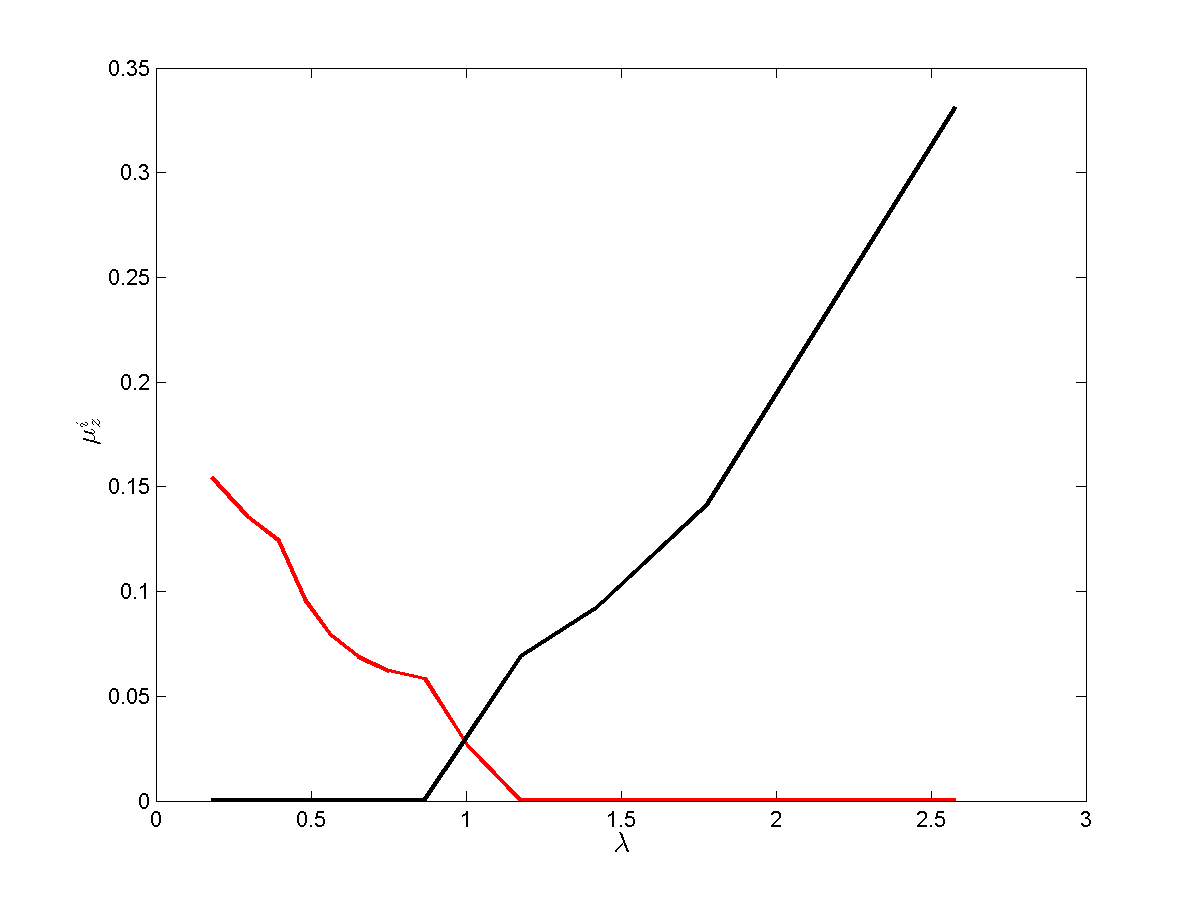
\includegraphics[scale=0.4]{Matlab/PrivateInformation/Plots/BindingMultipliers.png}

	\caption{ This figure plots the multiplier on the binding incentive
 constraint. The red line refers to $\mu^1_2$ - Agent 1 State $z_2$ and the
 black line refers to $\mu^2_1$ - Agent 2 state $z_1$. The dotted line is
 $\theta=\infty$ case}
	\label{fig:BindingMultipliers}
\end{figure} 
\end{frame}


\begin{frame}
\frametitle{Optimal time 0 - Consumption Menu- Irrelevance of $\theta$}
\emph{Since the binding mechanics of $\mu$ are independent of $\theta$, we have that the initial period consumption plan as a function of $\lambda$ has the same property }

\begin{figure}[htbp]
\centering
	  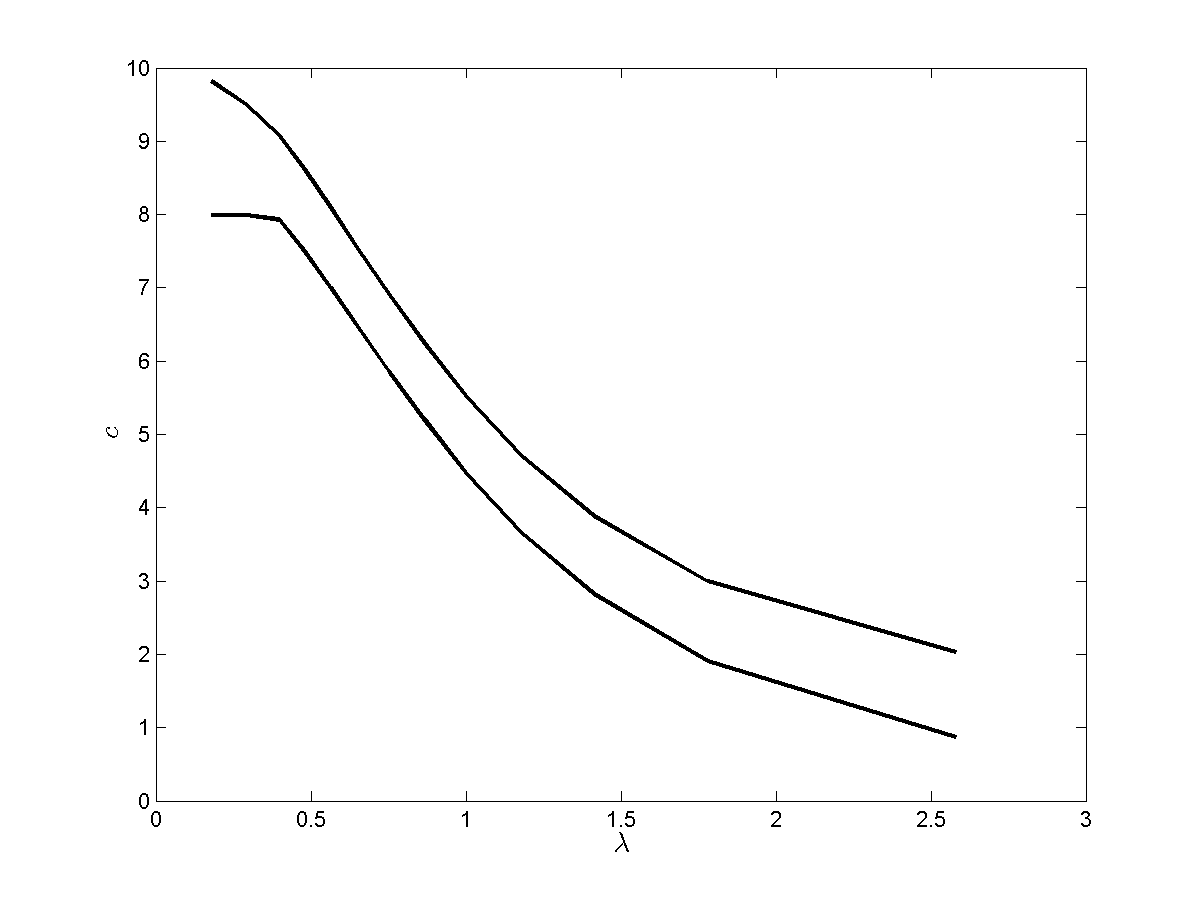
\includegraphics[scale=0.4]{Matlab/PrivateInformation/Plots/CompOptContractCons.png}

	\caption{This plot shows the time-0 consumption plan as a function of $\lambda$. The dotted line represents $\theta=\infty$}
	\label{fig:CompOptContractCons}
\end{figure} 
\end{frame}


\begin{frame}
\frametitle{FOC}
Let $\lambda^*(v,z)=Q^*_v(v,z)$
\begin{subequations}

\begin{equation}
\small c_0(1)^{-\gamma}\tilde{P}^1(1|z\_)-\mu^1_{z_2}[c_0(1)-\Delta]^{-\gamma}-[y-c_0(1)]^{-\gamma}(\lambda+\mu^2_{z_1})=0
\end{equation}
\begin{equation}
\small c_0(2)^{-\gamma}[\tilde{P}^1(2|z\_)+\mu^1_{z_2}]-\lambda[y-c_0(2)]^{-\gamma}\tilde{P}^2(2|z\_)+\mu^2_{z_1}[y-c_0(2)+\Delta]^{-\gamma}=0
\end{equation}

\begin{equation}
\small 
-\lambda^*[1,1]\tilde{P}^1(1|z\_)+\lambda\tilde{P}^2(1|z\_)+\mu^1_{z_2} \lambda^*[1,2]+\mu^2_{z_1}=0
\end{equation}

\begin{equation}
\small 
-\lambda^*[2,2]\tilde{P}^1(2|z\_)+\lambda\tilde{P}^2(2|z\_)-\mu^1_{z_2} \lambda^*[2,2]-\mu^2_{z_1}=0
\end{equation}

\end{subequations}
\begin{subequations}
\begin{equation}
\small u[c_0(2)]+\delta Q^{0}[2,2]\geq u[c_0(1)+\Delta]+\delta Q^{0}[1,2]
\end{equation}
\begin{equation}
\small u[y-c_0(1)]+\delta \bar{v}^{*}(1)\geq u[y-c_0(2)+\Delta]+\delta \bar{v}^{*}(2)
\end{equation}
\end{subequations}
\end{frame}
\end{document}	



